\section{Introduction}\label{Sec:intro}

\kom{Einleitung umschreiben; sample bias als aufhänger rausschmeißen, genau so wie das Gebru bsp! ergo den gesamten ersten absatz; stattdessen induktionsproblem und dann dataset shift als instanz davon (s. Corfielf, projection and probability)}

In recent years \textit{data} has become a hot topic \kom{to (for?)} the broader public, exceeding its natural habitat of science and computer programming by far. Some proclaimed it to be the oil/gold of the $21{th}$ century. A reason for the rush lies in the availability of data and the development of new technologies and methods, which enables us to design algorithms that \textit{learn} from data. The emerging scientific field is known as Machine Learning (ML), Some even see the advent of a new age of science:
\begin{quote}
	The new availability of huge amounts of data, along with the statistical tools to crunch these numbers, offers a whole new way of understanding the world. Correlation supersedes causation, and science can advance even without coherent models, unified theories, or really any mechanistic explanation at all.\footnote{\url{https://www.wired.com/2008/06/pb-theory/}}
\end{quote}
To slow down a little the above quoted author we could simply ask him about the problem of induction, the question whether it is possible to infer a generally valid law based on single observations. Presumed we go bird watching and observe a 100 swans, all of them in white plumage. We could then draw the following two inductive conclusions:	
\begin{quote}
	(C1) All swans observed so far were white. Therefore all swans are white. $(F(a_1),\dots,F(a_n) \Rightarrow \forall x: F(x))$ \\
	(C2) All swans observed so far were white. Therefore the next observed swan will be white. $(F(a_1),\dots,F(a_n) \Rightarrow F(a_{n+1}))$
\end{quote} 
This poses two questions regarding justification: how do we justitfy to generalize about some objects $x$ features $F$ based on $n$ observations of a particular instance $(F(a_1),\dots,F(a_n) $; and how do we justify the assumption, that future observations $F(a_{n+1})$ are going to occur the same as past ones. The problem of induction forms one of the fundamental problems in the domain of Epistemology and Philosophy of Science. The reason we bring this up\kom{,} is to remark that (statistica) learning from data faces the same problems  as any field operating with inductive inferrence. Regarding ML we could then alter $(C1)$ in the following way\begin{quote}
	(C3) All observations $x_i$ for feature $x$ fall within the range of $[a,b]$. Therefore the model learns $x \in [a,b]$. \\
	(C4) All observations $x_i$ for feature $x$ fall within the range of $[a,b]$. Therefore the model predicts $x \in [a,b]$ for $x_{n+1}$.
\end{quote} 
The reasoning of C3 and C4 does not seem problematic, one could insist and give us referral to all those well-functioning ML models and applications. But, especially when it comes to real world ML applications, the following problem is very common: the data $x \in [a,b]$ used for training the underlying model is not strictly (or not at all represenative) of the data $x \in [c,d]$ on which the model will be tested on in the end by the user. \kom{Den Satz umdrehen, also das die Testdaten abweichen und nicht die Trainingsdaten} This violation of C3 and C4 is called dataset shift \citep{moreno2012unifying}. More technically speaking, dataset shift appears when training and test joint distributions are different \citep{quionero2009dataset}. Moreno et al. identify three main types of dataset shift, covering a shift in the independent variables (\textit{Covariate shift}), in the target variable (\textit{Prior probability shift}) or in the relationship between the two (\textit{Concept shift}) [\kom{Eigennamen nicht kursiv?}]. In this paper we will focus on the first of the three shifts, Covariate shift. 



The theme of this book raises the interesting question of how to encode further refined background knowledge to allow the accurate transfer of learning to take place. To do so in too domain-specific a way risks too much human involvement. We would prefer not to have to hand code background knowledge for each new situation. Ideally, we would even be able to learn the relevant invariances using general purpose algorithms.



%There are more critical voices, too \kom{(i.e. Rahimi, Vapnik, \dots)}. Some of them even come from the heartland of data; there was for instance the incident around Google's star ethics researcher Timnit Gebrus fall out from Google due to her participation in a paper on large scale language models. Besides remarking negative environmental aspects of these models, the authors critcize projects as Google's GPT3 regarding the data which is used for their training. One negative aspect of their data gathering is that these models will "fail to capture the language and the norms of countries and peoples that have less access to the internet and thus a smaller linguistic footprint online."\footnote{ As the paper is not officially published yet, I rely on \url{https://www.technologyreview.com/2020/12/04/1013294/google-ai-ethics-research-paper-forced-out-timnit-gebru/}} Therefore wealthier countries will be overrepresented in the data gathering, \kom{rendering} the training sample \textit{biased}. Only taking into account the technical dimension of this aspect, leaving out political, ethical and others, this illustrates a problem which should be familiar to everyone \kom{practically} enageged with data analysis and machine learning: Sample Selection Bias.

In machine learning (ML) the above sketched problem appears frequently in a similar shape: in a practical ML application the data used for training the underlying model is not strictly (or not at all represenative) of the data on which the model will be tested on in the end by the user. Biased training data can then cause so called \textit{dataset shift} \citep{moreno2012unifying}. More technically speaking, dataset shift appears when training and test joint distributions are different \citep{quionero2009dataset}. There are three main types of dataset shift \citep{moreno2012unifying}, covering a shift in the independent variables (\textit{Covariate shift}), in the target variable (\textit{Prior probability shift}) or in the relationship between the two (\textit{Concept shift}) [\kom{Eigennamen nicht kursiv?}]. In this paper we will focus on the first of the three shifts, Covariate shift. 

%In machine learning (ML) this problem is often encountered in the form of \textit{dataset shift}, which is mostly caused by sample selection bias  \citep{moreno2012unifying}. In general the problem is shaped similarly to the above sketched: in a practical ML application the data used for training the underlying model is not strictly (or not at all represenative) of the data on which the model will be tested on in the end by the user. Technically speaking, dataset shift appears when training and test joint distributions are different \citep{quionero2009dataset}. 

In this case the values of the covariates $X$ causally determine the class label $Y$. A shift then occurs, if the distribution of one or more of the covariates $X_{ts}$ in the test data significantly changes compared to $X_{tr}$ in the training data. A good example would be credit scoring, as the information on the potential customer, characterized by the covariates, determines the credit score $Y$. For further illustration we take a look at \citep[Sec.~8.2]{wang2020deontological}. There a credit scoring model is employed based on the \kom{taiwanese }UCI Credit Data Set. The authors then \kom{remark} a sample bias for the variable ``Repayment status'', as the data appears to be very noisy for cases with $overdue > 3$. In a simplified two-feature test case (with covariates ``marital status"\ and ``April repayment") their model then yields the output visualized in Fig. \ref{Fig:gup2}.
{\large{Austauschen mit fig4: observed default rate; Text entsprechend ändern}}

\begin{figure}[htb!]
	\centering
	\begin{minipage}{0.45\textwidth}
		\centering
		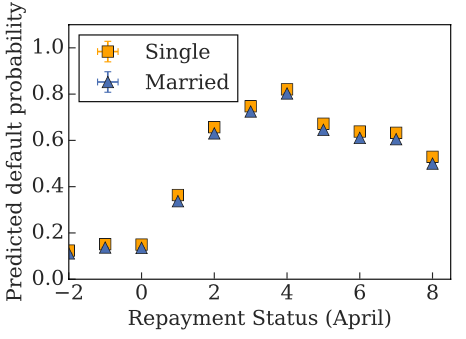
\includegraphics[width=1\textwidth]{gup2} % first figure itself
		\caption{\kom{first figure}}
		\label{Fig:gup2}
	\end{minipage}\hfill
	\begin{minipage}{0.45\textwidth}
		\centering
		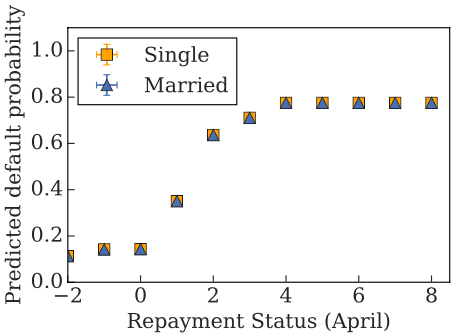
\includegraphics[width=1\textwidth]{gup1} % second figure itself
		\caption{\kom{second figure}}
		\label{Fig:gup1}
	\end{minipage}
\end{figure}

Fig. \ref{Fig:gup2} shows that customers, who are 5 or 6 month overdue, are assigned a lower score than those, who are only 2 months overdue. This means, borrowers are penalized by the score for paying back in time. The underlying bias most likely results from the training data only containing 122 cases of $overdue > 3$, leaving those cases underrepresented in a training set of 30.000 observations. To mitigate the bias of the estimator, which can be modeled as covariate shift, Wang and Gupta supplement their model with a \textit{mononicity shape constraint}. In Fig. \ref{Fig:gup1} we see a more consistent behaviour of the estimator, as the shape constraint permits to integrate prior knowledge into the model. For their experiment the authors used a nonlinear generalized additive model, respectively a TensorFlow Lattice (TFL) calibrated linear model. \kom{Noch zwei drei sätze zu tfl cal models}

The goal of this paper is to explore/\kom{examine}, whether lattice based and shape constraint models can be applied to reduce covariate shift. [...] \\
First theory, what happens in the lattice? Then experiment: genauer vorgang siehe \ref{Sec:Exp}; das brint uns zu dem result, dass die lattice methode eingeschränkt nutzbar ist.

Outline of the paper:\\
	{\it The paper is organized as follows. The next section describes related literature regarding this\&that. Section \ref{Sec:Method}} describes the  \ref{Sec:Results} presents the results. Finally, Section
		\ref{Sec:Conc} concludes.

%\begin{itemize}
%	
%	\item What is the subject of the study? Describe the
%	economic/econometric problem.
%	
%	\item What is the purpose of the study (working hypothesis)?
%	
%	\item What do we already know about the subject (literature
%	review)? Use citations: \cite{garcia2009lattice}
%	
%	\item What is the innovation of the study?
%	
%	\item Provide an overview of your results.
%	
%	\item Outline of the paper:\\
%	{\it The paper is organized as follows. The next section describes related literature regarding this\&that. Section \ref{Sec:Method}} describes the  \ref{Sec:Results} presents the results. Finally, Section
%		\ref{Sec:Conc} concludes.
%	
%	\item The introduction should not be longer than 4 pages.
%	
%\end{itemize}